En este Capítulo se abordan los conceptos básicos en los que se sustenta este trabajo, se busca mostrar de esta manera la postura conceptual de este objeto de estudio. En primer lugar, en la Sección \ref{sec:rm} se exploran los formalismos relacionados a la robótica móvil, además de los sistemas de medición como parte de la percepción de los estados internos y externos del robot aplicado al mismo. Para la Sección \ref{sec:na} se presentan un par de avances históricos importantes de la navegación autónoma dentro de la robótica móvil y las perspectivas actuales de la misma junto con los propios esquemas que buscan cuantificar la autonomía en los vehículos. La Sección \ref{sec:vi} se enfoca en la visión artificial, y en particular se exploran al final los sistemas de visión tridimensional, haciendo énfasis en los sensores RGB-D, tomando como punto de partida su uso dentro de la robótica móvil. Para finalizar el capítulo, en la Sección \ref{sec:con} se presentan las estrategias de control más usadas para este tipo de vehículos, se plantean los principales enfoques y se encuadra al {\it visual servoing} junto con sus características primarias.
\section{Robótica móvil}
\label{sec:rm}
A pesar de que existen un gran número de registros históricos acerca de autómatas que fueron elaborados por personajes que van desde Herón de Alejandría hasta Leonardo Da Vinci, la robótica es una rama del conocimiento joven en realidad, pues no se consolidó como ciencia hasta el siglo XX. En primera instancia la palabra robot se acuñó en la obra {\it Rossum's Universal Robots} de Carel Capek, la palabra proviene del idioma checo y en ese idioma se suele usar de manera coloquial para designar a un sirviente; en la cultura popular surgieron lo robots como personajes que podían realizar las tareas que a los humanos llegan a resultar de gran dificultad, y con la aparición de las tres leyes de la robótica de Isaac Asimov en {\it I, Robot}, se establecían las pautas a las que los fabricantes debían someter a los robots de la vida real.
\par La robótica se divide en las ramas de robótica de manipuladores y robótica móvil, siendo esta última la de interés en este trabajo. Desde el punto de vista más general, se define al robot móvil como aquel que es capaz de cambiar su posición sin estar sujeto a un solo punto. Las aplicaciones de los robots móviles son en realidad amplias, pues pueden ser usados en tareas de exploración, búsqueda y rescate, automatización de procesos, vigilancia, investigación científica y agricultura, por sólo mencionar algunas. Los robots, antes de alcanzar su grado de desarrollo actual, atravesaron un largo proceso de evolución y desarrollo. De ser mecanismos teleoperados, han llegado a adquirir rasgos que les brindan autonomía a través de acciones que les permiten medir características del entorno, calculando y actuando a partir de ello.
\subsection{Locomoción}
\label{ssec:loc}
Existen diferentes posibilidades de lograr el desplazamiento de un robot móvil, incluyendo (pero no limitando): Rodar, caminar, saltar, trepar, nadar, volar, etc. De acuerdo al medio en el que se desplaza se pueden clasificar en: Acuático, terrestre, aéreo e híbrido (combinando al menos dos de los medios).
\begin{table}[htbp!]
	\caption{Tipos de ruedas empleados en robótica móvil.}
	\label{tab:ruedas}
	\begin{center}
		\begin{tabular}{|p{3cm}|p{7cm}|p{4cm}|}
			\hline
			{\bf Tipo de rueda} & {\bf Grados de libertad} & {\bf Ejemplo}\\
			\hline
			Estándar 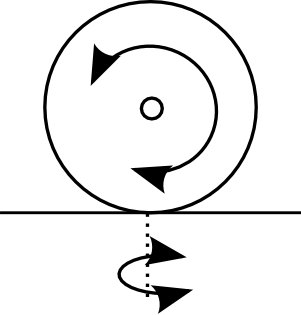
\includegraphics[width=2.5cm]{./Figuras/REstan.png} & Dos:
			\begin{compactitem}
				\item Rotación alrededor de su eje.
				\item Rotación alrededor de su punto de contacto con el suelo.
			\end{compactitem} & Rueda de carretilla\\
			\hline
			Castor 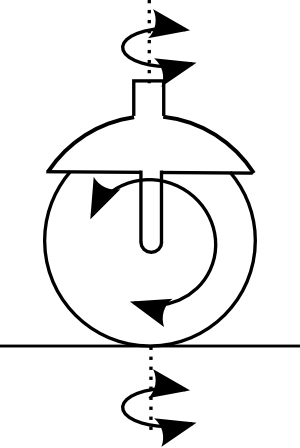
\includegraphics[width=2.5cm]{./Figuras/Castor.png} & Tres:
			\begin{compactitem}
				\item Rotación alrededor de su eje.
				\item Rotación alrededor de su punto de contacto con el suelo.
				\item Rotación en el eje de la rueda.
			\end{compactitem} & Silla de oficina\\
			\hline
			Omnidireccional (Sueca) 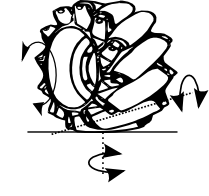
\includegraphics[width=2.5cm]{./Figuras/Sueca.png} & Tres:
			\begin{compactitem}
				\item Rotación alrededor de su eje.
				\item Rotación alrededor de su punto de contacto con el suelo.
				\item Rotación alrededor de sus  rodamientos.
			\end{compactitem} & Kuka youBot\\
			\hline
			Esférica 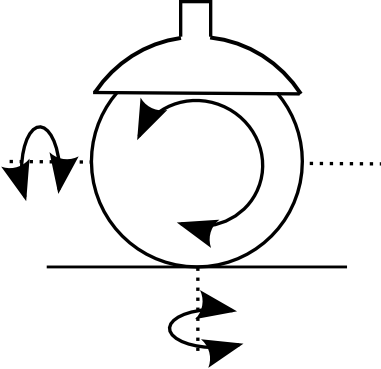
\includegraphics[width=2.5cm]{./Figuras/REsfera.png} & Tres:
			\begin{compactitem}
				\item Rotación en cualquier dirección.
				\item Rotación alrededor de su punto de contacto con el suelo.
			\end{compactitem} & Rodamiento de bolas\\
			\hline
		\end{tabular}
	\end{center}
\end{table}
\vspace*{-0.6cm}
\par En el caso de los robots móviles terrestres, los hay con configuraciones basadas en patas (buscando emular el movimiento de los animales, insectos y humanos), orugas y ruedas; de forma similar, dentro de los robots móviles con ruedas se pueden ordenar de acuerdo al tipo de ruedas empleados, y a su vez en la configuración con la que estas funcionan en conjunto para el gobierno de la plataforma. De \cite{barrientossotelovictorricardoRobotsMovilesEvolucion} se ha tomado la Figura \ref{fig:configuraciones}, que ilustra las principales configuraciones de robots móviles, mientras que de \cite{corellnikolausIntroductionAutonomousRobots2014} se tomó y adaptó la Tabla \ref{tab:ruedas} para enumerar los tipos de ruedas máxime usados junto con sus características y usos; la información mostrada en esta Sección se apoya en estas dos bibliografías junto con \cite{fernandoRoboticaControlRobots2011}.
\begin{figure}[htbp!]
	\centering
	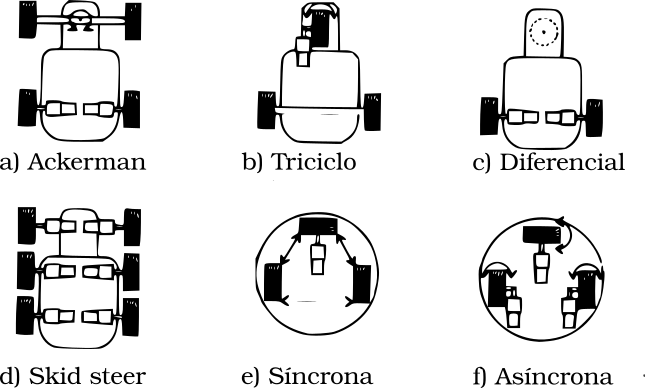
\includegraphics[width=0.45\textwidth]{./Figuras/Configuraciones}
	\caption{Principales configuraciones de robots móviles con ruedas.}
	\label{fig:configuraciones}
\end{figure}
\par El desplazamiento de los RMR se da gracias al uso de actuadores, en muchas ocasiones eléctricos. Exceptuando a los motores a pasos (que no resultan convenientes para propulsar un vehículo eléctrico por su baja relación de velocidad), los motores eléctricos de corriente directa e imán permanente son los actuadores más empleados para la locomoción en los RMR, y estos se pueden encontrar a su vez en dos clasificaciones: Con escobillas y sin escobillas.
\par Por motivos prácticos, los motores eléctricos son usados en conjunto con cajas de engranes para reducir su velocidad y aumentar su par; asimismo, al integrar en el sistema un codificador rotatorio\footnote{Dispositivo de naturaleza electromecánica usado para traducir la posición angular de un eje a un código digital.}, es posible conocer la posición y la velocidad del motor para cada instante de tiempo. A estos motores se les conoce como {\it servomotores}, y su control requiere suministrar una serie de pulsos con diferente duración en milisegundos para obtener diferente posición angular; o bien distintos anchos de pulso en milisegundos para distintas velocidades angulares.
\subsection{Odometría}
La odometría es el estudio de la estimación de la posición de los robots móviles durante la navegación. Su estudio implica tomar la información de los sensores presentes en la plataforma para obtener los cambios de posición de la misma a lo largo del tiempo. 
\par El concepto básico es desarrollar un modelo matemático para establecer la manera en que los comandos enviados a las extremidades del robot (ruedas, orugas, patas, etc.) inducen el movimiento de la plataforma. Este término también se usa a veces para referirse a la trayectoria que ha recorrido uno de estos vehículos, dejando la posibilidad de emplear diferentes tipos de sensores para obtener la posición a lo largo del tiempo, como lo son los codificadores rotatorios, sistemas de visión (llamado odometría visual), brújulas, giroscopios, acelerómetros, GPS, etc.
\par La idea fundamental de la odometría se encuentra en la integración de información incremental obtenida a partir del movimiento a lo largo del tiempo, y esto tiene como desventaja una acumulación de errores debido a los propios sensores empleados, en particular la acumulación de errores de orientación (lo que causa grandes inexactitudes en la estimación de la posición), a la larga los errores aumentarán de manera proporcional a la distancia recorrida por el robot. No obstantes estas limitaciones, la odometría es una parte importante del sistema de navegación de un robot, debe usarse junto con medidas del posicionamiento absolutas para proporcionar una estimación de la posición más fiable. Los errores que se mencionan se pueden agrupar en dos categoría:
\paragraph{Errores sistemáticos:}
\begin{itemize}
	\item Los diámetros de las ruedas no son iguales.
	\item Mala alineación de las ruedas.
	\item Baja resolución en la tasa de muestreo de los sensores.
\end{itemize}
\paragraph{Errores no sistemáticos:}
\begin{itemize}
	\item Desplazamiento en suelos desnivelados.
	\item Desplazamiento sobre objetos inesperados que se encuentren en el suelo.
	\item Patinaje de las ruedas (debido a suelos resbaladizos, sobre-aceleración, derrapes, fuerzas externas, falta de un punto de contacto con el suelo).
\end{itemize}
\par Se vuelve un asunto importante distinguir entre los errores sistemáticos y los no sistemáticos para mitigar la incertidumbre en la odometría; en particular los errores sistemáticos son graves, pues se acumulan constantemente; por su parte los errores no sistemáticos generan problemas que pueden aparecer de manera espontánea, y pueden causar errores significativos en la estimación de la posición (un ejemplo se puede dar cuando el robot pasa por encima de un objeto que se encuentra en el suelo).
\subsection{Percepción}
\label{ssec:per}
Es fundamental para cualquier sistema de navegación poseer la habilidad de medir los estados internos del vehículo, además de poder percibir su entorno. Para adquirir el conocimiento del ambiente, los sistemas robóticos emplean diferentes tipos de sensores, y esta actividad se combina con la interpretación de las mismas en función de variables físicas, todo esto bajo la consideración que cada tipo de sensor tiene ventajas y limitaciones inherentes que necesitan ser compensadas. Los sensores involucrados pueden arrojar mediciones de índole externa e interna\footnote{Estas categorías son conocidos como {\it propiocepción} y {\it exterocepción} en el argot biológico.}. El tipo de sensores disponibles para el robot móvil determina de manera directa las estrategias de control disponibles para la navegación autónoma de la plataforma. En \cite{siegwartIntroductionAutonomousMobile2011} y \cite{corellnikolausIntroductionAutonomousRobots2014} se da una descripción más amplia de los principales medios de percepción en la robótica, además se complementa con la tesis \cite{b.VisualHomingCarlike2005}. 
\subsubsection{Sensores internos}
\label{sssec:si}
Esta categoría de sensores es la encargada de la percepción de los estados propios del robot, y abarca la medición del nivel de carga de las baterías, la posición de los actuadores del robot, velocidad, aceleración y torque de los mismos, por sólo mencionar algunas. Entre los sensores propioceptivos de mayor relevancia dentro de los RMR se encuentra el codificador rotatorio: el cual permite conocer la posición angular en los ejes de los motores, y con base en ello se vuelve posible obtener la distancia recorrida y la velocidad de la plataforma, esto al conocer el radio de la rueda y el tiempo entre muestras. El codificador rotatorio, en el caso de un funcionamiento óptico, cuenta con una rueda que tiene ranuras claras y ranuras oscuras, de manera que cuando la rueda se encuentre girando, un emisor óptico se encontrará trabajando de manera continua y por lo tanto el receptor óptico alternará valores lógicos de $1$ y $0$. En la Figura \ref{fig:CRO} se ilustra el funcionamiento de un codificador rotatorio de funcionamiento óptico como el descrito con anterioridad.
\begin{figure}[htbp!]
	\centering
	\includegraphics[width=0.5\textwidth]{./Figuras/Encoder}
	\caption{Disco de codificador rotatorio de funcionamiento óptico.}
	\label{fig:CRO}
\end{figure}
\subsubsection{Sensores externos}
\label{sssec:se} 
Esta jerarquía de sensores es la encargada de la percepción de los aspectos exteriores del robot, y envuelve a la localización de las características del entorno que permiten la ubicación del robot y de los objetos circundantes en el espacio de trabajo. Dentro de esta categoría se encuentran las balizas, las brújulas, los sistemas de posicionamiento global (GPS), los sensores de distancia (ultrasónicos, LIDAR\footnote{Sistema basado en laser que brinda una imagen del entorno a partir de la detección y medición de la distancia alrededor}, etc.), y los sistemas de visión artificial.
\par En esta clase se puede contar con la información provista por los sensores de navegación inercial (denominadas también IMU), que involucran la medición de seis grados de libertad que se dan con la aceleración a lo largo de los ejes $x$, $y$ y $z$, además de los ángulos de \textit{alabeo}, \textit{cabeceo} y \textit{guiñada}. De manera interna, la medición de estas variables se da gracias a los MEMs.
\par Los sensores externos aportan más confianza en las mediciones que los sensores internos porque miden ángulos y distancias de manera directa, lo que resulta más eficiente que hacerlo a partir de la lecturas de velocidad y aceleración. A pesar de ello, estos sensores pueden presentar problemas (mismos que a su vez se pueden mitigar al controlar las condiciones de operación de la plataforma robótica), como lo son:
\begin{itemize}
	\item Requiere una línea de visión para poder operar.
	\item Interferencias por obstrucción o reflexión (en el caso de sensores de visión y de distancia), y por la presencia de estructuras metálicas o campos magnéticos (en el caso de los sensores magnéticos).
\end{itemize}
\subsection{Restricciones holónomas y no-holónomas}
\label{ssec:rnh}
Los robots que usan sólo ruedas con tres grados de libertad son capaces de moverse libremente en el plano. En estos casos, la posición del robot está dada por dos valores que definen la posición y otro que define la orientación. Cada vehículo de ruedas se encuentra sujeto a constantes cinemáticas que lo reducen en su movilidad local, dejando intacta la posibilidad de alcanzar configuraciones arbitrarias con maniobras apropiadas. Si se considera un sistema mecánico cuya configuración $\mathbf{q}$ está descrita por un vector de coordenadas generalizadas, y el espacio de todas las posibles configuraciones del robot coincide con $\mathds{R}^{n}$. El movimiento del sistema que está representado por la evolución de $\mathbf{q}$ en el tiempo, debe estar sujeto a restricciones. Si las mismas pueden ser expresadas en la forma 
\[h_{i}(\mathbf{q})=0\quad i=1, \dots,k<n\]
se les llama holónomas (o integrables). Las restricciones holónomas por lo regular son el resultado de interconexiones mecánicas entre varios elementos del sistema. Por otra parte, las restricciones que involucran coordenadas generalizadas y velocidades en la forma
\[a_{i}(\mathbf{q}, \mathbf{\dot{q}})=0\quad i=1,\dots,k<n\]
son llamadas no-holónomas (también llamadas cinemáticas o no integrables). Las restricciones no-holónomas reducen la movilidad del sistema mecánico, perdiendo accesibilidad en el espacio de configuraciones. En sistemas con restricciones cinemáticas, el número de coordenadas que describe su configuración siempre es mayor que el número de grados de libertad que posee, y en principio ésta es la razón por la que se dificulta estacionar un vehículo en paralelo \cite{sicilianoRoboticsModellingPlanning2009}.
\subsection{Modelado cinemático}
\label{ssec:mc}
Partiendo de la noción de la rueda como un disco rodando en el plano, se puede obtener un modelo generalizado de los RMR a partir del más simple de ellos: El uniciclo.
\par Como se indica en la Figura \ref{fig:Uni}, la posición del robot en el plano se encuentra descrita, con respecto a un marco inercial, por las coordenadas generalizadas $\mathbf{q}=[x, y, \theta]^{T}$, donde el par $(x, y)$ representa las coordenadas de un punto arbitrario sobre el plano sagital\footnote{Plano perpendicular al suelo y en ángulo recto con el plano frontal, que divide al objeto en su mitad derecha e izquierda.} del robot, mientras que $\theta$ describe la orientación del robot con respecto al marco inercial.
\begin{figure}[htbp!]
	\centering
	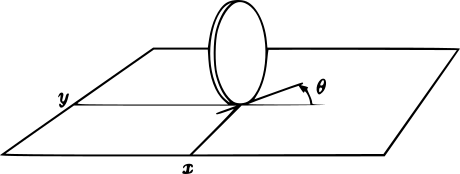
\includegraphics[width=0.5\textwidth]{./Figuras/Uniciclo}
	\caption{Coordenadas generalizadas para un disco rodando en el plano.}
	\label{fig:Uni}
\end{figure}
\par Para una rueda convencional, las restricciones cinemáticas implican que la velocidad del centro de la rueda es paralela a la plano de rotación ({\it condición de no deslizamiento}) y es proporcional a la velocidad de rotación de la rueda (i. e. {\it condición de balanceo puro}). La condición de balanceo puro para el disco se puede expresar como
\begin{equation}
	\dot{x}\sen\theta-\dot{y}\cos\theta=[\sen\theta, -\cos\theta, 0]\mathbf{\dot{q}}=0
\end{equation}
\par Lo que implica que la velocidad del punto de contacto es cero en la dirección ortogonal al plano sagital de la rueda. La línea que pasa a través del punto de contacto teniendo tal dirección se llama {\it línea de movimiento cero}. Con esto, se puede considerar la matriz
\[\mathbf{G(q)}=[\mathbf{g_{1}(q)}, \mathbf{g_{2}(q)}]=\left[
\begin{array}{cc}
\cos\theta & 0\\
\sen\theta & 0\\
0 & 1\\
\end{array}\right]\]
cuyas columnas $\mathbf{g_{1}(q)}$ y $\mathbf{g_{2}(q)}$ son, para cada $\mathbf{q}$, una base del espacio nulo asociado a las restricciones. Todas las velocidades generalizadas de $\mathbf{q}$ son por lo tanto una combinación lineal de $\mathbf{g_{1}(q)}$ y $\mathbf{g_{2}(q)}$. El modelo cinemático del uniciclo es, entonces
\begin{equation}
	\left[\begin{array}{c}
	\dot{x}\\
	\dot{y}\\
	\dot{\theta}\\
	\end{array}\right]=\left[\begin{array}{c}
	\cos\theta\\
	\sen\theta\\
	0\\
	\end{array}\right]v+
	\left[\begin{array}{c}
	0\\
	0\\
	1\\
	\end{array}\right]\omega
\end{equation}
donde las entradas $v$ y $\omega$ son la velocidad lineal y angular, como corresponde \cite{sicilianoRoboticsModellingPlanning2009}.
\par La configuración de robot móvil que se aproxima más al uniciclo es la configuración diferencial (Figura \ref{fig:configuraciones}c). Entre otras, una de las desventajas de una configuración diferencial es la dependencia de una rueda castor --que se comporta pobremente a altas velocidades y dificulta las estrategias de conducción-- además de requerir de la sincronización de ambos motores para conducirse a la misma velocidad exacta. Por fortuna, las mismas desventajas pueden ser mitigadas por el mecanismo empleado por los autómoviles, que es conducido por un sólo motor y puede gobernar las ruedas laterales a través de un servomecanismo. Esta configuración es conocida como {\it plataforma Ackerman} (Figura \ref{fig:configuraciones}a), donde cada rueda en la configuración Ackerman es su propio punto de pivote y el sistema se encuentra restringido de tal manera que todas las ruedas del vehículo van en una circunferencia con un punto central en común, evitando así derrapes. A bajas velocidades, se puede emplear el modelo de un triciclo o el de una bicicleta para aproximar el comportamiento de la configuración Ackerman. La bicicleta tiene una rueda trasera fija al cuerpo del vehículo, y rota con respecto al eje vertical de la rueda delantera para conducir el vehículo \cite{corellnikolausIntroductionAutonomousRobots2014}.
\par En un robot móvil, si se prolonga con una recta al eje perpendicular a cada rueda, el punto en el que se da la intersección es llamado Centro Instantáneo de Rotación (CIR); este es el punto de referencia sobre el cual el vehículo sigue una trayectoria circular, y entonces su velocidad angular está dada por
\begin{equation}\label{eq:giro}
	\dot{\theta}=\frac{v}{R}
\end{equation}
de manera que por relaciones geométricas se conoce que el radio de giro $R$ se obtiene por $R=L/\tan(\varphi)$, teniendo a $L$ como la distancia entre los ejes frontal y trasero del vehículo, y a $\varphi$ como el ángulo de gobierno para el vehículo, mismo que típicamente se encuentra limitado mecánicamente y su máximo valor determina el valor de $R$. Tomando como ejemplo la Figura \ref{fig:CIR}, las líneas punteadas muestran la dirección a lo largo de la cual las ruedas no se pueden mover, cruzándose en el CIR del vehículo \cite{sicilianoRoboticsModellingPlanning2009, corkeRoboticsVisionControl2017}.
\begin{figure}[htbp!]
	\centering
	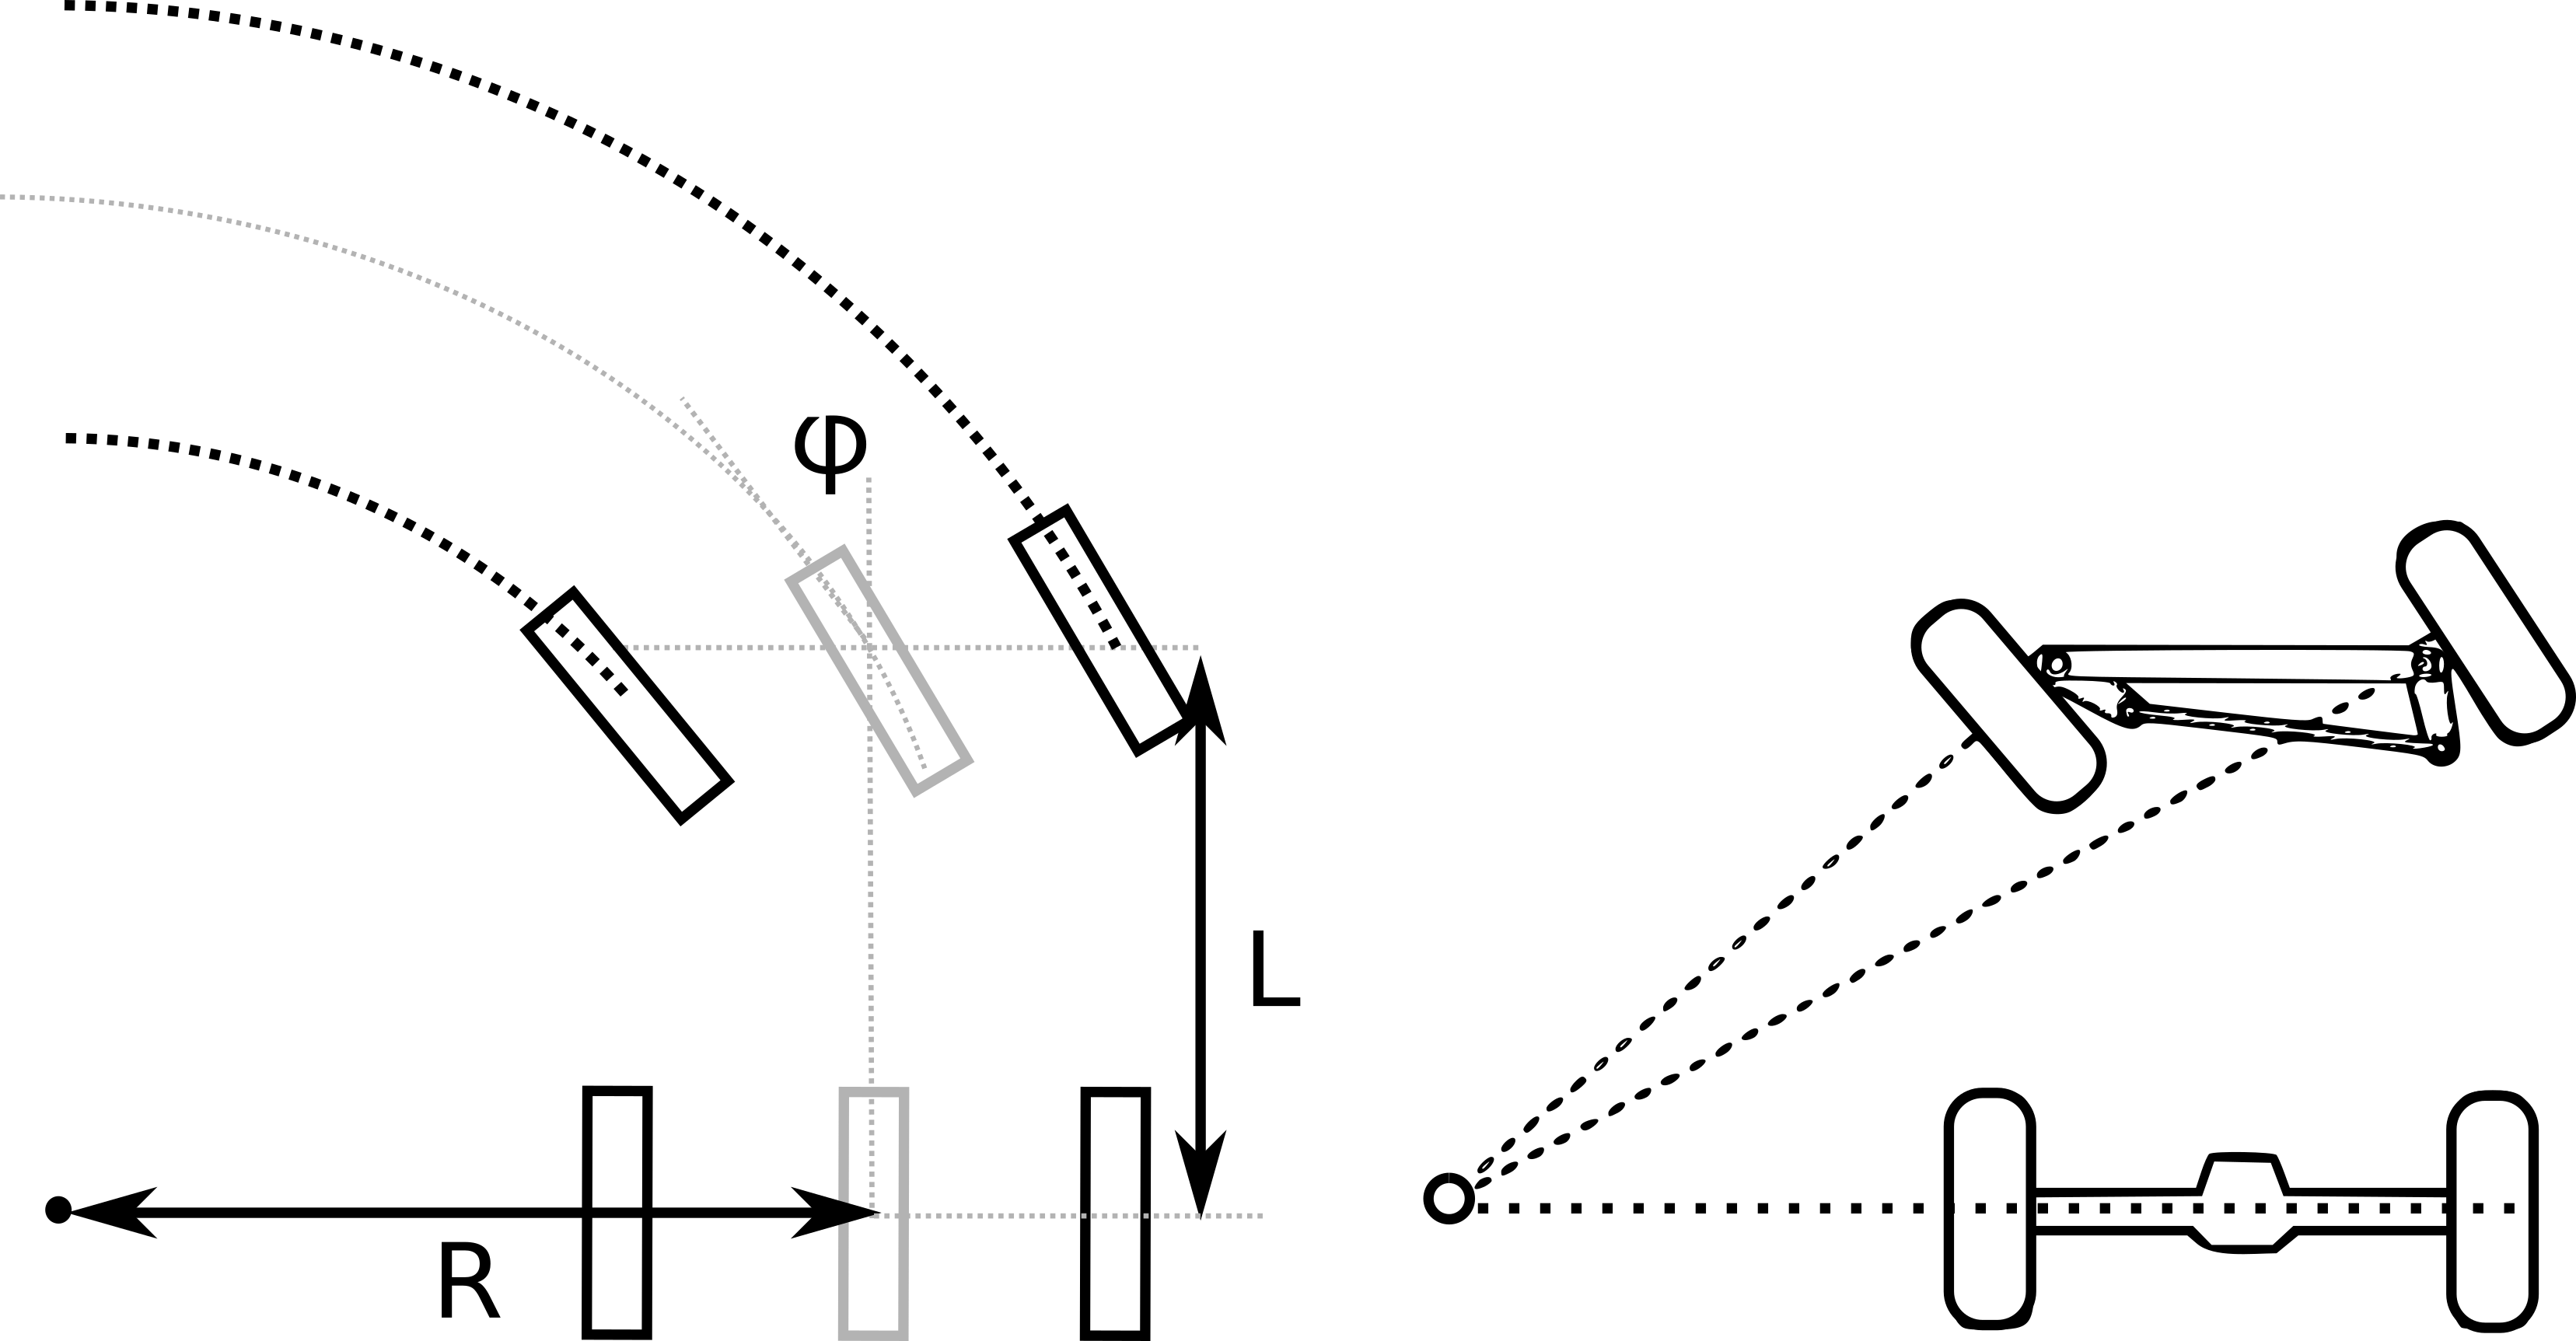
\includegraphics[width=0.5\textwidth]{./Figuras/Ackerman}
	\caption{Derecha: Cinemática del mecanismo de gobierno utilizado por los automóviles. Izquierda: Mecanismo de un vehículo Ackerman.}
	\label{fig:CIR}
\end{figure}
\par Gerasimos Rigatos y Krishna Busawon proponen en \cite{rigatosRoboticManipulatorsVehicles2018} un modelo dinámico del vehículo de cuatro ruedas en la configuración Ackerman y otro para un vehículo de dos ruedas para la configuración de bicicleta, además proponen una linealización de estos dos modelos, junto con algunas estrategias de control tanto lineales como no lineales. En dichos modelo se consideran los deslizamientos longitudinal y lateral del vehículo, así como la guiñada, y son representados por las ecuaciones \eqref{eq:long}, \eqref{eq:lat} y \eqref{eq:yaw} respectivamente.
\begin{equation} \label{eq:long}
	-mV(\dot{\beta}+\dot{\varPsi})\sen(\beta)+m\dot{V}\cos(\beta)=f_{x}
\end{equation}
\begin{equation} \label{eq:lat}
	mV(\dot{\beta}+\dot{\varPsi})\cos(\beta)+m\dot{V}\sen(\beta)=f_{y}
\end{equation}
\begin{equation} \label{eq:yaw}
	I\ddot{\varPsi}=T_{z}
\end{equation}
Donde $m$ es la masa del vehículo, $\beta$ representa el ángulo entre el vehículo y el plano sagital, $V$ es el vector velocidad del vehículo, $\varPsi$ es el ángulo de guiñada, $f_{x}$ es la fuerza agregada en el eje $x$, $f_{y}$ es la fuerza agregada en el eje $y$, y $T_{z}$ es el par agregado alrededor del $z$. Estas ecuaciones se pueden escribir de forma matricial como
\begin{equation}
	\left[\begin{array}{ccc}
	-\sen(\beta) & \cos(\beta) & 0\\
	-\cos(\beta) & \sen(\beta) & 0\\
	0 & 0 & 1
	\end{array}\right]
	\left[\begin{array}{c}
	mV(\dot{\beta}+\dot{\varPsi})\\
	m\dot{V}\\
	I\ddot{\varPsi}
	\end{array}\right]=\left[\begin{array}{c}
	f_{x}\\
	f_{y}\\
	T_{z}
	\end{array}\right]
\end{equation}
\par Asimismo, G. Oriolo et al. en \cite{laumondRobotMotionPlanning1998} desarrollan un modelo cinemático para los robots móviles con configuración Ackerman, y el modelo se ha basado a su vez en la bicicleta. Este último trabajo será de más ayuda que el de Gerasimos Rigatos, y se explorará a detalle en la Sección \ref{sec:mc}.
\section{Navegación autónoma}
\label{sec:na}
Algunas de las primeras aproximaciones a la navegación autónoma se remontan al primer par de robots móviles autónomos de la historia. {\it Elmer} y {\it Elsie}\footnote{Siglas en inglés para Electro Light Sensitive Internal External} (Elsie  en la Figura \ref{fig:ELSIE}), un par de tortugas robóticas que fueron construidas a finales de la década de 1940 por William Grey Walter, quien eraun neurocientífico de la universidad de Bristol. Este par de tortugas estaban diseñadas para buscar una fuente de luz sin tener información previa de la posición de la misma \cite{w.greyMachineThatLearns1951}. Durante la década de 1960 apareció el robot {\it Shakey} (Figura \ref{fig:Shakey}) del SRI\footnote{Instituto de Investigación de Stanford}, que era capaz de crear un mapa de su entorno para planear una trayectoria a un punto de destino predefinido \cite{nilsonn.j.ShakeyRobot1984}.
\begin{figure}[htbp!]
	\centering
	\begin{subfigure}[h]{0.4\textwidth}
		\centering
		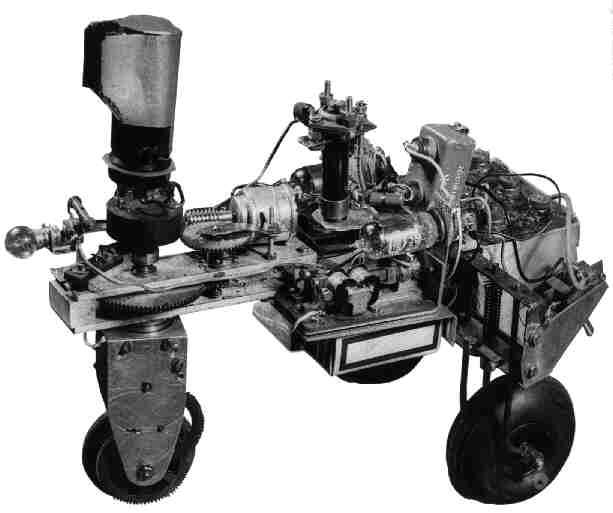
\includegraphics[width=\textwidth]{./Figuras/ELSIE}
		\caption{Robot Elsie sin su caparazón.}
		\label{fig:ELSIE}
	\end{subfigure}
	\begin{subfigure}[h]{0.4\textwidth}
		\centering
		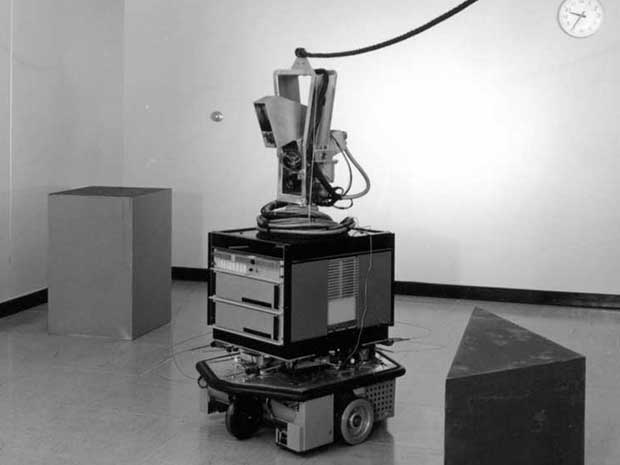
\includegraphics[width=\textwidth]{./Figuras/Shakey}
		\caption{Robot Shakey.}
		\label{fig:Shakey}
	\end{subfigure}
	\caption{Antecedentes de la robótica móvil}
\end{figure}
\par Una de las funciones más importantes de un robot móvil es poder moverse hacia algún lugar, mismo que puede ser especificado en términos de alguna característica del ambiente (como seguir la luz, seguir paredes, etc.) o en función de alguna coordenada geográfica de referencia. Una estrategia se basa en tomar mediciones simples del mundo y reaccionar a lo medido. Los sistemas de navegación reactiva pueden ser simples y a la vez veloces, ya que el sistema de medición está conectado directamente a la acción. Los sistemas que crean mapas y razonan acerca de estos requieren más recursos; no obstante, son capaces de realizar tareas más complejas \cite{corkeRoboticsVisionControl2017}.
\par Para la robótica móvil, la tarea de navegación representa una ciencia en sí misma por la gran cantidad de técnicas relacionadas con alcanzarla. La localización del robot en el plano, además de la manera en que se ve posibilitado para actuar en éste (esquivando obstáculos, guiándose por diferentes características  del entorno, seguir una ruta, etc.) permiten llevar a la navegación teleoperada o preprogramada a una navegación autónoma.
\par En el contexto urbano actual, se plantean los autos del mañana como sistemas autónomos, i. e. robots móviles autónomos que integren una variedad de sensores para su localización espacial y la consecuente navegación reactiva. Según lo expuesto en \cite{heinrichPlanningUniversalOnRoad2018}, estos sistemas incorporan una gran variedad de beneficios, listados a continuación:
\begin{itemize}
	\item Un vehículo habilitado para conducirse por sí mismo en el escenario y actuar en caso de peligro, puede disminuir el 90 \% de los accidentes de tránsito causados por el ser humano.
	\item Un vehículo habilitado para ir a altas velocidades y cerca de otro sin peligro, reduce el consumo de combustible y emisión de gases a la atmósfera.
	\item Si un vehículo puede moverse de manera autónoma en un terreno, o entrar en un campo minado, o cualquier otra misión peligrosa, el número de individuos en riesgo se decrementa.
\end{itemize}
Además en el mismo texto se sugiere que la operación de los vehículos inteligentes involucra:
\begin{itemize}
	\item El monitoreo del ambiente en torno al vehículo.
	\item Comunicación con la infraestructura de tránsito y otros vehículos.
	\item Percibir la geometría del carril y del camino.
	\item Reconocer los señalamientos de tránsito.
	\item Distinguir el estado de los semáforos.
\end{itemize}
\par Para estas tareas, la visión artificial juega un rol básico. Por un lado, el camino puede ser detectado por sistemas LIDAR (depende de su construcción), sin embargo para detectar los carriles se requiere la visión artificial; la detección de las señales de tránsito se puede realizar tomando en consideración los colores, geometría y reconocimiento de los símbolos presentes dentro de los límites del señalamiento; la detección del estado del semáforo es un problema que involucra reconocer el color y la intensidad del mismo, y por la luz ambiental puede resultar problemático si la misma llega a opacar la luz del semáforo \cite{broggiIntelligentVehicles2008}.
\par La SAE\footnote{Sociedad de Ingenieros Automotrices.} publicó un manual de referencia con los diferentes niveles de automatización \cite{saeTaxonomyDefinitiosTerms2014} para vehículos, el cual contiene las métricas para situar a un vehículo dentro de alguno de los 6 niveles de automatización planteados, mismos que se resumen en la Tabla \ref{tab:niveles}, y van desde la nula automatización (representada por el nivel 0) hasta su antípoda: la nula intervención humana en el proceso de conducción (nivel 5 de esta clasificación).
\begin{center}
	\begin{longtable}{|p{1cm}|p{3.5cm}|p{5.5cm}|p{5.5cm}|}
		\caption{Niveles de automatización propuestos por la SAE}
		\label{tab:niveles}
		\endfirsthead
		\caption*{{\bf Tabla \ref{tab:niveles}:} Continuación}
		\endhead
		\endfoot
		\endlastfoot
		\hline
		{\bf Nivel} & {\bf Designación} & {\bf Rol del conductor} & {\bf Rol de la computadora}\\ 			\hline\hline
		0 & Sin automatización & \begin{compactitem}
			\item Monitoreo del entorno.
			\item Ejecutar las tareas de giro, aceleración y freno.
		\end{compactitem} & \begin{compactitem}
			\item No aplica.
		\end{compactitem}\\ 
			\hline
		1 & Conducción asistida & \begin{compactitem}
			\item Monitoreo del entorno.
			\item Realizar el control lateral o longitudinal según corresponda.
			\item Desactivar la conducción asistida si se requiere.
		\end{compactitem} & \begin{compactitem}
			\item Realizar el control lateral o longitudinal según corresponda.
		\end{compactitem}\\
			\hline
		2 & Automatización parcial & \begin{compactitem}
			\item Monitoreo del entorno.
			\item Determinar el momento adecuado para la activación de la automatización parcial.
			\item Supervisar la conducción del sistema de automatización parcial.
			\item Desactivar la automatización parcial si se requiere.
		\end{compactitem} & \begin{compactitem}
			\item Ejecutar las tareas de giro, aceleración y freno.
		\end{compactitem}\\
			\hline
		3 & Automatización condicional & \begin{compactitem}
			\item Determinar el momento adecuado para la activación de la automatización condicional.
			\item Supervisar la conducción del sistema de automatización condicional.
			\item Desactivar la automatización condicional si se requiere.
		\end{compactitem} & \begin{compactitem}
			\item Monitoreo del entorno.
			\item Ejecutar las tareas de giro, aceleración y freno.
		\end{compactitem}\\
			\hline
		4 & Automatización alta & \begin{compactitem}
			\item Determinar el momento adecuado para la activación de la automatización condicional.
			\item Supervisar la conducción del sistema de automatización condicional.
			\item Desactivar la automatización condicional si se requiere.
		\end{compactitem} & \begin{compactitem}
			\item Monitoreo del entorno.
			\item Ejecutar las tareas de giro, aceleración y freno.
			\item Permitir la activación sólo bajo los casos para los cuales ha sido diseñado.
			\item Desactivarse hasta que el conductor humano tome el control.
		\end{compactitem}\\
			\hline
		5 & Automatización completa & \begin{compactitem}
			\item No aplica.
		\end{compactitem} & \begin{compactitem}
			\item Monitoreo del entorno.
			\item Ejecutar las tareas de giro, aceleración y freno.
		\end{compactitem}\\
			\hline
		\end{longtable}
	\end{center}
\section{Visión}
\label{sec:vi}
Con muy pocas y contadas excepciones, todos los animales cuentan con ojos, y estos están asociados a un poderoso (e igualmente complejo) sistema de procesamiento paralelo para el volumen de información percibida, mismo sistema que ha tomado millones de años de constante evolución para alcanzar su estado de desarrollo actual. La visión es una poderosa habilidad para la navegación en los animales y en seres humanos, y es por ello que se posiciona como una buena elección para la adquisición de información cualitativa que permite la navegación de los robots móviles. Los sistemas de visión forman parte de los sensores exteroceptivos, pero al abarcar por sí mismo un amplio campo de investigación, en esta Sección se describirá por separado de lo expuesto en la \autoref{ssec:per}. La redacción de esta Sección se apoya sobre todo haciendo referencia a Peter Corke, Richard Szeliski y a Heredia Favieri en \cite{corkeRoboticsVisionControl2017},  \cite{szeliskiComputerVisionAlgorithms2011} y \cite{herediafavieriReconocimientoObjetosImagenes2015}, como corresponde.
\begin{figure}[htbp!]
	\centering
	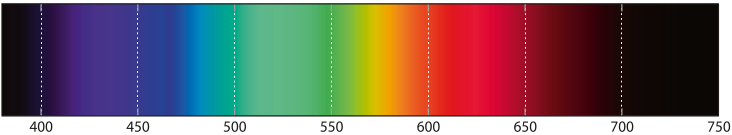
\includegraphics[width=0.7\textwidth]{./Figuras/Espectro}
	\caption{Colores del espectro visible en función de su longitud de onda.}
	\label{fig:espectro}
\end{figure}
\par Fue hacia el año 1670 cuando Sir Isaac Newton se dio cuenta de que la luz blanca es el resultado de la combinación de luces de diferentes colores. Ahora se sabe que cada uno de esos colores está asociado con una longitud de onda y a una frecuencia en el espectro electromagnético, pudiendo observar nosotros como humanos un pequeño rango de éste espectro, abarcando longitudes de onda que abarcan de manera aproximada entre 400 y 700 nm aproximadamente, como se puede observar en la Figura \ref{fig:espectro}.
\begin{figure}[htbp!]
	\centering
	\begin{subfigure}[h]{0.25\textwidth}
		\centering
		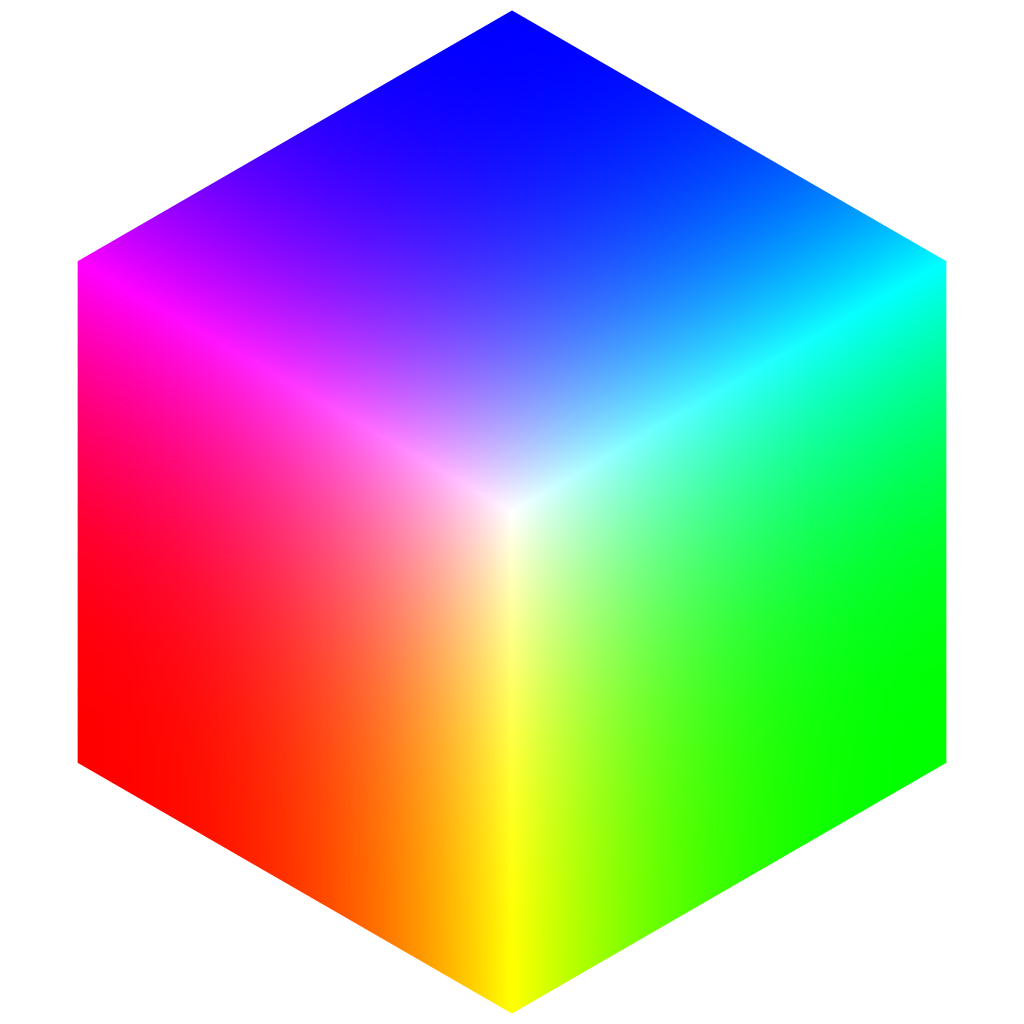
\includegraphics[width=\textwidth]{./Figuras/RGB}
		\caption{Modelo RGB.}
		\label{fig:RGB}
	\end{subfigure}
	\begin{subfigure}[h]{0.25\textwidth}
		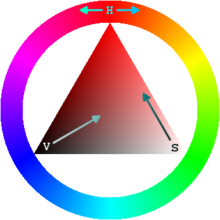
\includegraphics[width=\textwidth]{./Figuras/HSV}
		\caption{Modelo HSV.}
		\label{fig:HSV}
	\end{subfigure}
	\begin{subfigure}[h]{0.25\textwidth}
		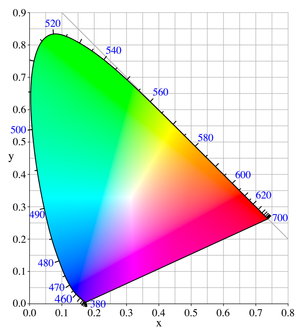
\includegraphics[width=\textwidth]{./Figuras/CIE}
		\caption{Modelo CIE.}
		\label{fig:CIE}
	\end{subfigure}
	\caption{Algunos de espacios de color más empleados.}
\end{figure}
\par El modelo más empleado en la actualidad para la representación de los colores es el que utiliza como base al Rojo, Verde y Azul (RGB por sus siglas en inglés), y es el más natural al aproximarse a la manera en la que el ojo humano capta la luz como colores positivos y negativos. En la Figura \ref{fig:RGB} se muestra la manera en que al combinar estos colores entre sí en diferentes intensidades se obtiene como resultado otro color diferente, siendo el blanco la combinación de los tres en la máxima intensidad, y el negro la ausencia de luz. Sin embargo, el espacio de color RGB no es el único que puede ser utilizado para representar los colores en la luz, y algunos de estos ejemplos son el HSV y el CIE (Figuras \ref{fig:HSV} y \ref{fig:CIE}.), aunque se debe decir que existen otros tantos y además variaciones de los mismos.
\begin{figure}[htbp!]
	\centering
	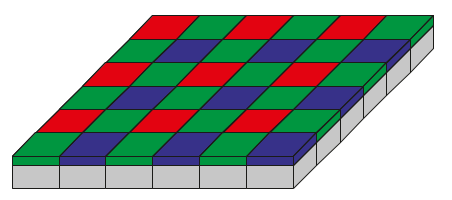
\includegraphics[width=0.5\textwidth]{./Figuras/Bayer}
	\caption{Patrón de Bayer para una cámara.}
	\label{fig:Bayer}
\end{figure}
\par Las imágenes, computacionalmente hablando, se componen de la intensidad lumínica que se percibe en cada uno de los elementos de un arreglo bidimensional de receptores sensibles a una longitud de onda específica. La información provista por la imagen equivale a la captura de una escena en un instante, y representa los valores de la intensidad que llega a cada uno de los receptores lumínicos de la cámara. En una cámara digital que trabaja en el espacio de color RGB, por ejemplo, se cuenta con un patrón de receptores lumínicos llamado patrón de Bayer (Figura \ref{fig:Bayer}), y estos receptores pueden existir como semiconductores con tecnología CCD o CMOS.
\begin{figure}[htbp!]
	\centering
	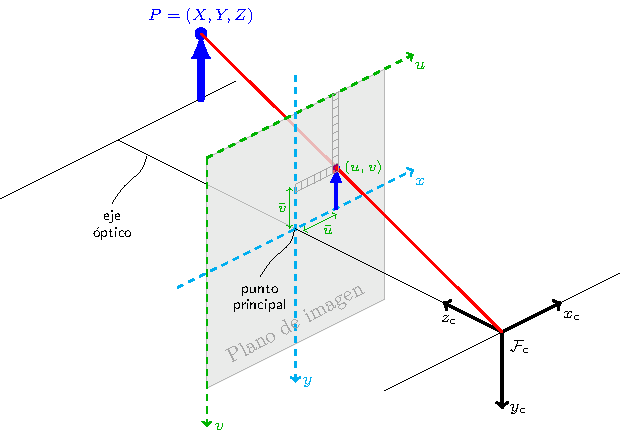
\includegraphics[width=0.6\textwidth]{./Figuras/Perspectiva}
	\caption{Proyección de perspectiva tridimenional a bidimensional.}
	\label{fig:Per}
\end{figure}
\par Gracias a la información obtenida por las imágenes, es posible conocer características importantes de los objeto que se encuentran en el escenario capturado por la cámara, tales como el color, la forma, la posición o la orientación, por mencionar algunas. El proceso de formación de imágenes en un ojo o una cámara involucra la proyección de un mundo tridimensional en una superficie bidimensional. La información de profundidad está perdida cuando se trabaja sólo con una cámara, por lo que no se puede distinguir al punto más cercano del más lejano en una imagen. La transformación de imágenes desde un espacio tridimenensional a uno bidimensional se conoce como proyección de perspectiva, y en la Figura \ref{fig:Per} se muestra un diagrama que expone la naturaleza de la transformación, en la misma el cuadro sombreado con una línea verde punteada rodeándolo representa la imagen bidimensional, en donde un punto $P=(X, Y, Z)$ adquiere coordenadas $p=(u, v)$, pudiendo percibir de esta manera la pérdida de la información de profundidad en la proyección de perspectiva.
\par Además de la pérdida de información provocada por la proyección de perspectiva, surge una incertifumbre cuando la imagen que se observa sufre deformaciones debido a diferentes factores, como la ubicación de la cámara con respecto al objeto a observar. Ante todo existen dos acciones por las que se pueden producir alteraciones en la imagen:
\begin{enumerate}
	\item La interpolación de los niveles intensidad de los pixeles.
	\item Una transformación espacial que define la reubicación de los pixeles en la imagen.
\end{enumerate}
\par La primera de estas acciones, la interpolación de los niveles de intensidad en los pixeles, es un problema que puede originarse por problemas de la iluminación de la escena o del objeto, mientras que por otra parte puede surgir por la sensibilidad de los receptores. En realidad estos problemas en la interpolación pueden ser resueltos al controlar la manera en que se toma la captura de la escena, buscando controlar la iluminación de acuerdo a las características que se busca capturar.
\par En la segunda de las acciones, que implica la perspectiva de la cámara con respecto a la escena, se involucran a las transformaciones espaciales. Estas también llamadas modificaciones, preservan los ángulos mientras que las distancias entre los puntos cambian en una proporción fija y los objetos mantienen una forma similar (triángulos similares, círculos similares, etc.). Estas transformaciones contienen el escalamiento, la traslación y la rotación. De manera general se usa la operación matricial de la Ecuación \eqref{eq:simi} para calcular las transformaciones de similaridad:
\begin{equation}\label{eq:simi}
	\left[\begin{array}{c}
	x'\\
	y'\\
	1
	\end{array}\right]=
	\left[\begin{array}{ccc}
	a\cos\theta & -a\sen\theta & x_{t}\\
	a\sen\theta & a\cos\theta & y_{t}\\
	0 & 0 & 1
	\end{array}\right]
	\left[\begin{array}{c}
	x\\
	y\\
	1
	\end{array}\right]
\end{equation}
\par Si a las transformaciones de similaridad las acompañan las transformaciones de deslizamiento y escalado no uniforme, se obtienen las transformaciones afines, de las cuales se destaca que los objetos que son observados conservan las líneas paralelas. La operación que definen las transformaciones afines se hayan en la Ecuación \eqref{eq:afin}, conteniendo los componentes de seis grados de libertad correspondientes a los coeficientes $a_{00}$, $a_{01}$, $a_{10}$, $a_{11}$.
\begin{equation}\label{eq:afin}
	\left[\begin{array}{c}
	x'\\
	y'\\
	1
	\end{array}\right]=
	\left[\begin{array}{ccc}
	a_{00} & a_{01} & x_{t}\\
	a_{10} & a_{11} & y_{t}\\
	0 & 0 & 1
	\end{array}\right]
	\left[\begin{array}{c}
	x\\
	y\\
	1
	\end{array}\right]
\end{equation}
\par Junto con la identificación de las transformaciones espaciales que sufre la imagen, existen algunas otras operaciones que son de importancia y a la vez muy comunes dentro del procesamiento de imágenes. Se toman como elementos al filtrado de imágenes y la detección de sus características.
\par Al ser las imágenes señales bidimensionales, la teoría de filtros sobre señales unidimensionales puede ser extendida para describir el funcionamiento de los filtros en dos dimensiones. Existen filtros tipo pasa alto, pasa bajo, pasa banda y rechaza banda por mencionar sólo algunos. El proceso de filtrado puede llevarse a cabo en el dominio de la frecuencia o en el dominio del espacio. Por tanto, se pueden definir los principales objetivos que se consiguen con el filtrado de imágenes:
\begin{itemize}
	\item {\bf Suavizar la imagen:} Reducir la cantidad de variaciones de intensidad entre pixeles vecinos.
	\item {\bf Eliminar ruido:} Eliminar aquellos pixeles cuyo nivel de intensidad sea muy diferente al de sus vecinos y cuyo origen pueda estar tanto en el proceso de adquisición de la imagen como en el de transmisión.
	\item {\bf Realzar bordes:} Destacar los bordes que se localizan en una imagen.
	\item {\bf Detectar bordes:} Detectar los pixeles donde se produce un cambio brusco de la intensidad.
\end{itemize}
\par Si se requiere realizar el filtrado de la imagen en el dominio de la frecuencia, entonces se emplea la transformada de Fourier sobre la imagen. De manera general, el procedimiento empleado para aplicar los filtros en el dominio de la frecuencia a una imagen es el siguiente:
\begin{enumerate}
	\item Se aplica la transformada de Fourier (FFT\footnote{Transformada Rápida de Fourier.}).
	\item El resultado se multiplica por la función del filtro que ha sido escogido (Butterworth, Bessel, Chebyshev, etc.).
	\item Se aplica la transformada inversa de Fourier (IFFT\footnote{Transformada Inversa Rápida de Fourier.}) para devolver la imagen al dominio espacial.
\end{enumerate}
\par Mientras que para realizar el filtrado en el dominio del espacio, las operaciones se llevan a cabo de manera directa sobre los pixeles de la imagen, esto con el uso de núcleos de dimensión cuadrada cuyo objetivo es resaltar los cambios en la imagen. Durante el proceso se relaciona, para cada uno de los pixeles que conforman la imagen, un conjunto de pixeles próximos al pixel objetivo con la finalidad de obtener información útil relacionado con el tipo de filtro que se ha aplicado, lo cual permite actuar sobre el pixel concreto en que se está llevando a cabo el proceso de filtrado. A través del filtrado en el dominio del espacio se puede trabajar sobre la detección de características de imágenes como los bordes, siendo algunos de los más conocidos núcleos u operadores el Sobel, Prewitt, Roberts o Canny.
\par Adentrándose en las múltiples aplicaciones de Visión Artificial, existen múltiples operaciones que resultan útiles para el análisis de imágenes, y la detección de características. De la documentación de la librería OpenCV\cite{opencvOpenCVReferenceManual} se toma la Tabla \ref{tab:car}, donde se exponen algunos de los principales algoritmos para detección de características en imágenes.
\begin{center}
	\begin{longtable}{|l|l|}
		\caption{Principales algoritmos para detección de características empleados por OpenCV.}
		\label{tab:car}
		\endfirsthead
		\caption*{{\bf Tabla \ref{tab:car}:} Continuación.}
		\endhead
		\endfoot
		\endlastfoot
		\hline
		{\bf Tipo de operador} & {\bf Nombre del algoritmo}\\
		\hline
		\hline
		\multirow{5}{*}{}
		& Sobel\\ \cline{2-2}
		& Prewitt\\ \cline{2-2} 
		Detección de bordes & Deriche\\ \cline{2-2}
		& Roberts\\ \cline{2-2}
		& Canny\\ \hline
		\multirow{5}{*}{}
		& Harris\\ \cline{2-2}
		& Shi y Tomasi\\ \cline{2-2}
		Detección de esquinas & Curvas de nivel\\ \cline{2-2}
		& SUSAN\\ \cline{2-2}
		& FAST\\ \hline
		\multirow{4}{*}{}
		& Laplaciano del Gaussiano (LoG)\\ \cline{2-2}
		& Diferencia del Gaussiano (DoG)\\ \cline{2-2}
		Reconocimiento de regiones & Determinante del Hessiano (DoH)\\ \cline{2-2}
		& PCBR\\ \hline
		\multirow{2}{*}{}
		Transformada de Hough & Generalizada\\ \cline{2-2}
		& Probabilística\\ \hline
		\multirow{2}{*}{}
		Tensor estructural & Generalizado\\ \cline{2-2}
		& Probabilístico\\ \hline
		\multirow{3}{*}{}
		& Adaptación de figura afín\\ \cline{2-2}
		Detección de características afines invariantes & Harris afín\\ \cline{2-2}
		& Hessiano afín\\ \hline
		\multirow{5}{*}{}
		& SIFT\\ \cline{2-2}
		& SURF\\ \cline{2-2}
		Descripción de características & GLOH\\ \cline{2-2}
		& HOG\\ \hline
	\end{longtable}
\end{center}
\subsection{Visión tridimensional}
El mundo se compone de elementos tridimensionales y dinámicos, en él los hechos acontecen a alrededor en las dimensiones horizontal, vertical y en profundidad. Una imagen bidimensional aislada no da información suficiente en cuanto a la profundidad de los objetos en una escena, por lo que a grandes rasgos sería necesario definir la generación de un mundo tridimensional a través de tres componentes: el mundo de objetos tridimensionales, las fuentes de luz que componen y la cámara que observa la escena. De forma tradicional, durante gran parte del siglo XX y algunos años del siglo XXI se empleó la combinación de multiples cámaras para el cálculo de puntos tridimensionales a partir de las perspectivas individuales de cada una de las cámaras involucradas. Buscando de este modo emular el funcionamiento de la visión humana, se construyeron cámaras binoculares con disposición similar al acomodo de los ojos,  llamadas cámaras estereoscópicas. Un enfoque más moderno se da con la incorporación de los sensores RGB-D, que involucran la combinación de una cámara en el espacio de color RGB junto con un sensor de profundidad en la escena. Los siguientes dos apartados abarcan estos dos enfoques de visión tridimensional.
\subsubsection{Visión estéreo}
El concepto básico que se encuentra latente en la visión estéreo es la triangulación: Desde la ubicación de un punto de la escena, se forma un triángulo entre la correspondecia del mismo punto en las imágenes de las dos cámaras que toman la escena; conociendo la distancia existente entre las dos cámaras, además de los ángulos formados entre las cámaras y el punto de la escena, la distancia hasta el objeto puede ser determinada. La extracción de la estructura tridimensional de una escena a partir de imágenes estereoscópicas es un problema que ha sido estudiado ampliamente.
\par El funcionamiento esencial de las cámaras estereoscópicas tiene lugar en la geometría epipolar, la cual sólo tiene influencia de los parámetros intrínsecos de la cámara utilizada y su posición relativa, y es independiente de la estructura de la escena. Tal como se observa en la Figura \ref{fig:epi}, la escena de una cámara no es más que una traslación y una rotación de la imagen original.
\begin{figure}[htbp!]
	\centering
	\includegraphics[width=0.6\textwidth]{./Figuras/Epipolar}
	\caption{Modelo de geometría epipolar para cámara estereoscópica.}
	\label{fig:epi}
\end{figure}
\par En este punto inicia por dilucidarse la triangulación que es necesaria aplicar para obtener las coordenadas espaciales de un punto de la escena observado por ambas cámaras, esto a partir de las coordenadas planares de ambas cámaras. La desventaja principal de la visión estereoscópica se encuentra en el poder de cómputo necesario para poder manejar ambas imágenes como una sola y además realizar las operaciones de procesamiento necesarias. A pesar de esto, su uso es ampliamente extendido en general con procesos donde se requiere reducir costos.
\subsubsection{Sensores RGB-D}
Son muchos los sensores que se desarrollan en primer lugar para distintas aplicaciones diferentes antes de llegar a usarse en la robótica, tal es el caso de los sensores RGB-D, mismos que fueron desarrollados para la industria militar antes de pasar a la industria de los videojuegos (como el caso del Kinect de Microsoft), para de ahí expandirse a una amplia variedad de campos, incluyendo sus aplicaciones a la robótica. El Kinect (Figura \ref{fig:rgbd}) es un dispositivo que emplea una cámara como sensor RGB, además de un proyector de haces de luz infrarroja y un receptor (estos dos integran el sensor de profundidad). Las cámaras RGB-D proveen información de importancia acerca del entorno, pues a través de una nube de puntos y una imagen plana se vuelve posible tener un panorama tridimensional de alrededor; similar a lo que pudiera ser obtenido a partir de cámaras estéreo, con un costo de cómputo menor.
\begin{figure}[htbp!]
	\centering
	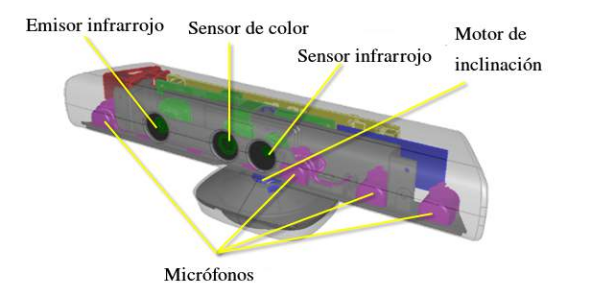
\includegraphics[width=0.6\textwidth]{./Figuras/RGB-D}
	\caption{Esquema de la configuración interna de un sensor RGB-D Kinect.}
	\label{fig:rgbd}
\end{figure}
\par Para el reconocimiento de objetos por medio de este tipo de sensores se emplean tres etapas: Extracción de puntos de interés, generación de descriptores y búsqueda de correspondencias. En general, la generación de descriptores se refiere a la extracción de representaciones significativas de los objetos a partir de observaciones como mallas poligonales o nubes de puntos. La imagen ya se ha descrito a lo largo de esta sección como una señal bidimensional, sin embargo quedan por definir las mallas poligonales y las nubes de puntos, mismas relaciones que son útiles para expresar el funcionamiento de los sensores RGB-D.
\paragraph{Malla poligonal:} Es una colección de vértices, ejes y caras que definen la forma de un objeto en tres dimensiones. Un vértice corresponde a un punto en el espacio, un eje es una conexión entre dos vértices, y una cara es un conjunto cerrado de ejes, siendo en general un triángulo o cuadrilátero. La densidad de una malla poligonal determina la resolución del objeto.
\paragraph{Nube de puntos:} Es una colección de puntos tridimensionales. Puede ser generada de forma artificial o provenir de capturas de elementos del mundo. Las coordenadas $\{x, y, z\}$ de cualquier punto de la nube están dadas con respecto a un sistema de coordenadas fijo. Si la nube representa datos del mundo, entonces el origen del sistema de coordenadas suele ser el sistema de captura utilizado. El valor de cada punto representa la distancia desde el origen hasta la superficie donde el punto fue capturado, pudiendo incluirse en cada punto datos como el color o la intensidad lumínica para esa pequeña sección de superficie en el objeto.
\par Para mostrar las diferencias en cuanto a su representación, en la Figura \ref{fig:elef} se muestra una malla poligonal y una nube de puntos, ambas del mismo objeto.
\begin{figure}[htbp!]
	\centering
	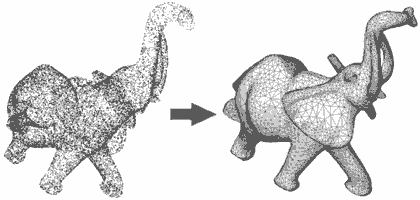
\includegraphics[width=0.5\textwidth]{./Figuras/Elefante}
	\caption{Derecha: Malla poligonal. Izquierda: Nube de puntos.}
	\label{fig:elef}
\end{figure}
\section{Control}
\label{sec:con}
El control consiste en manipular el valor de una variable para que el comportamiento se mantenga en un valor de referencia. En la actualidad, la teoría del control ha arrojado múltiples enfoques de control como la lógica difusa, redes neuronales, control clásico, control moderno o control robusto; sin embargo para llevar a cabo el control de un vehículo autónomo se considerarán tres enfoques:
\begin{itemize}
	\item Enfoque con Inteligencia Artificial.
	\item Enfoque sin Inteligencia Artificial (ingeniería manual).
\end{itemize}
\subsection{Enfoque con Inteligencia artificial}
La inteligencia artificial representa a la inteligencia llevada a cabo por máquinas. El término tal cual se aplica a las máquinas que son capaces de imitar las funciones cognitivas relacionadas con: Percibir, razonar, aprender y resolver problemas. La inteligencia artificial tiene aplicaciones en áreas como el control de sistemas, planificación automática, reconocimiento de patrones, etc. La máquina biológica que es capaz de realizar estas acciones es el cerebro a través de las neuronas, a partir de lo cual han surgido aproximaciones basadas en las mismas, y son llamadas neuronas artificiales. El agrupamiento de las neuronas --naturales o artificiales-- compone una red neuronal. La Figura \ref{fig:RNN} muestra la estructura general de una neurona natural en comparación de una neurona artificial con la Figura \ref{fig:RNA}.
\begin{figure}[htbp!]
	\centering
	\begin{subfigure}[h]{0.4\textwidth}
		\centering
		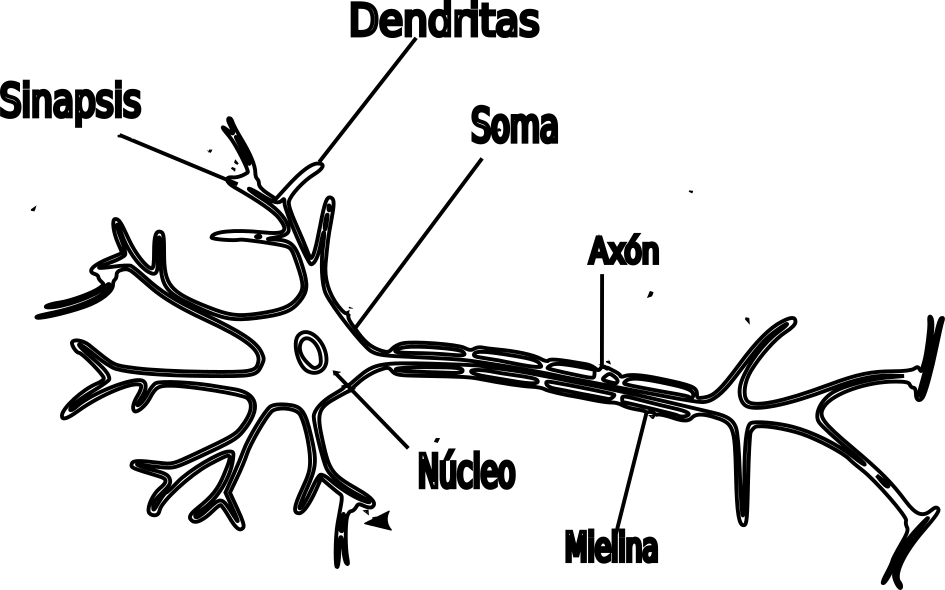
\includegraphics[width=\textwidth]{./Figuras/RNN}
		\caption{Representación esquemática de una neurona natural.}
		\label{fig:RNN}
	\end{subfigure}
	\begin{subfigure}[h]{0.5\textwidth}
		\centering
		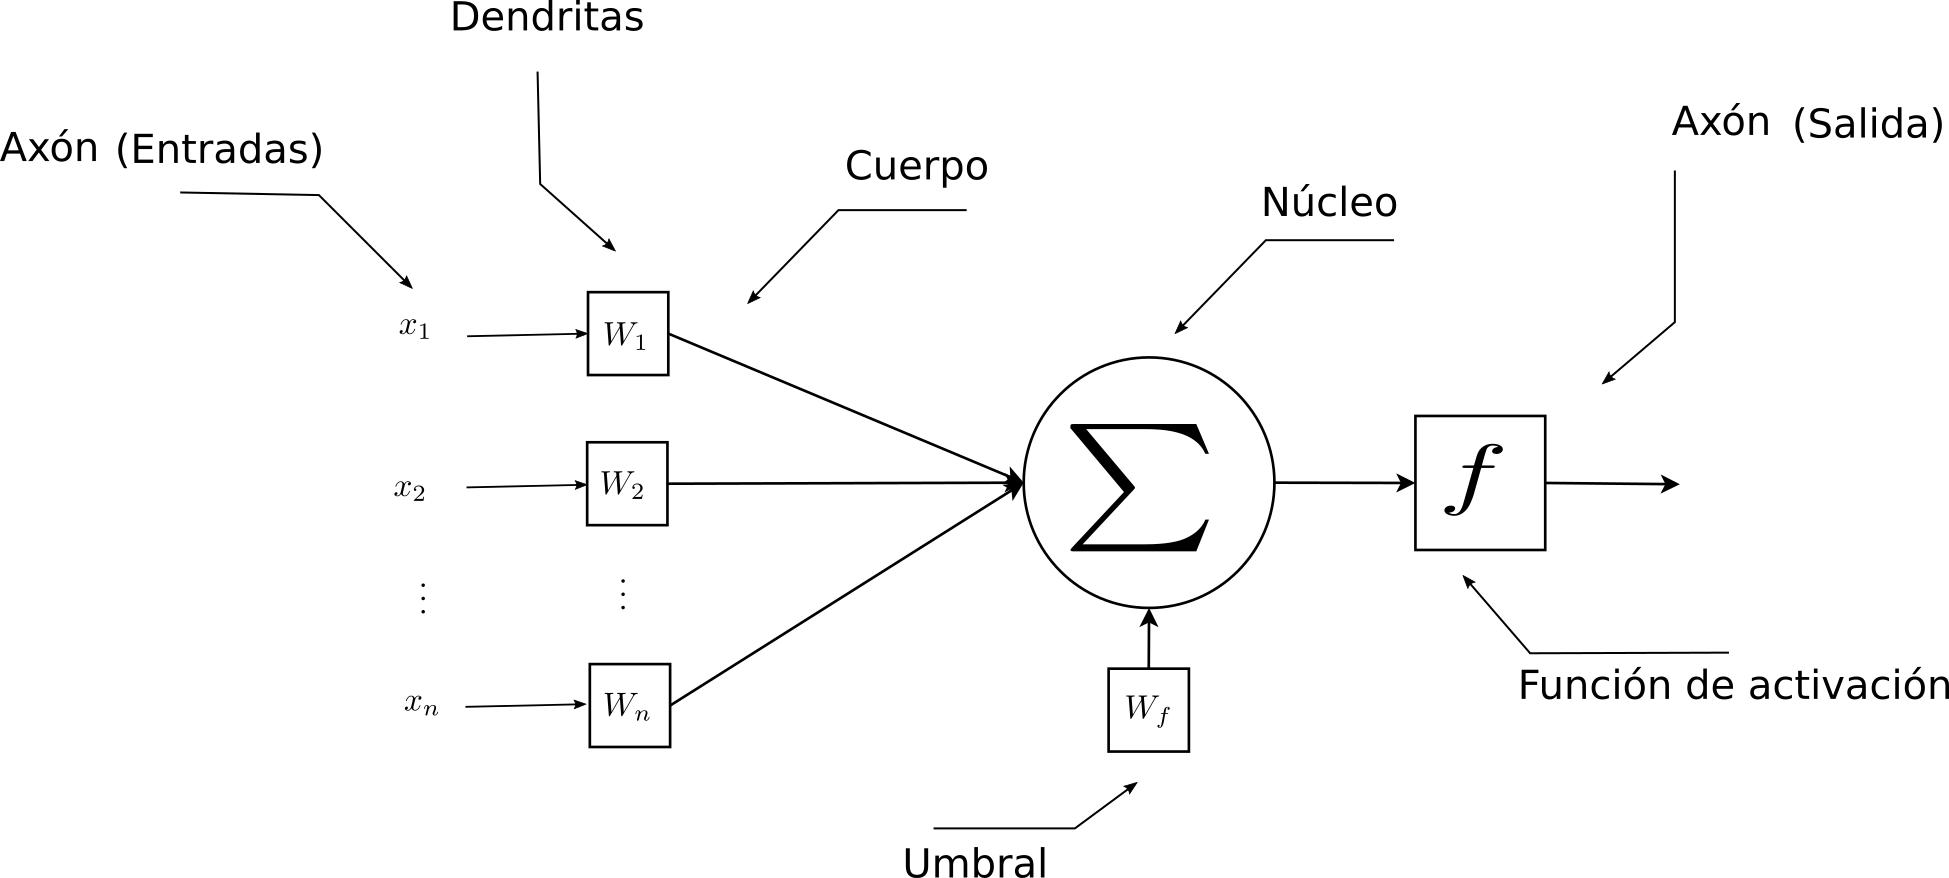
\includegraphics[width=\textwidth]{./Figuras/RNA}
		\caption{Representación esquemática de una neurona artificial.}
		\label{fig:RNA}
	\end{subfigure}
\end{figure}
\par Mediante el enfoque basado en IA no es necesario calcular la velocidad del vehículo ni el ángulo de giro en las ruedas usando ecuaciones matemáticas. Se propone una solución al problema de múltiples tareas para el gobierno del vehículo (lo que incluiría la evasión de obstáculos y el control de la orientación), y este enfoque permitiría llevar al vehículo desde su configuración inicial hasta su configuración final; es apoyado por el uso de redes neuronales, devolviendo como resultado el ángulo para la dirección de las ruedas y la velocidad del vehículo. Se emplea un agente inteligente\footnote{En Inteligencia Artficial, es una entidad capaz de percibir su entorno, procesar tales percepciones y responder o actuar en su entorno de manera racional.} que elige la mejor acción de acuerdo a los datos provistos por los sensores para la coordinación de los movimientos del robot. 
\subsection{Enfoque sin Inteligencia Artificial}
El enfoque sin Inteligencia Artificial usa el modelo matemático del vehículo para calcular la dirección de las ruedas necesaria para mantener el vehículo en el rumbo deseado, que es detectado a través de la visión artificial para las características del entorno. Uno de los métodos más populares en la teoría de control es el controlador PID (Proporcional-Integral-Derivativo). El controlador trabaja en un bucle que de manera continua calcula el valor de un error $e(t)$ como una diferencia entre la siguiente la orientación deseada y la actual (para este caso). A partir de esto la compensación es calculada y aplicada. El valor de correción $u(t)$ consiste en tres partes (Proporcional, Integral y Derivativa) y puede ser calculado a partir del error $e(t)$, como se aprecia en la Figura \ref{fig:PID}.
\begin{figure}[htbp!]
	\centering
	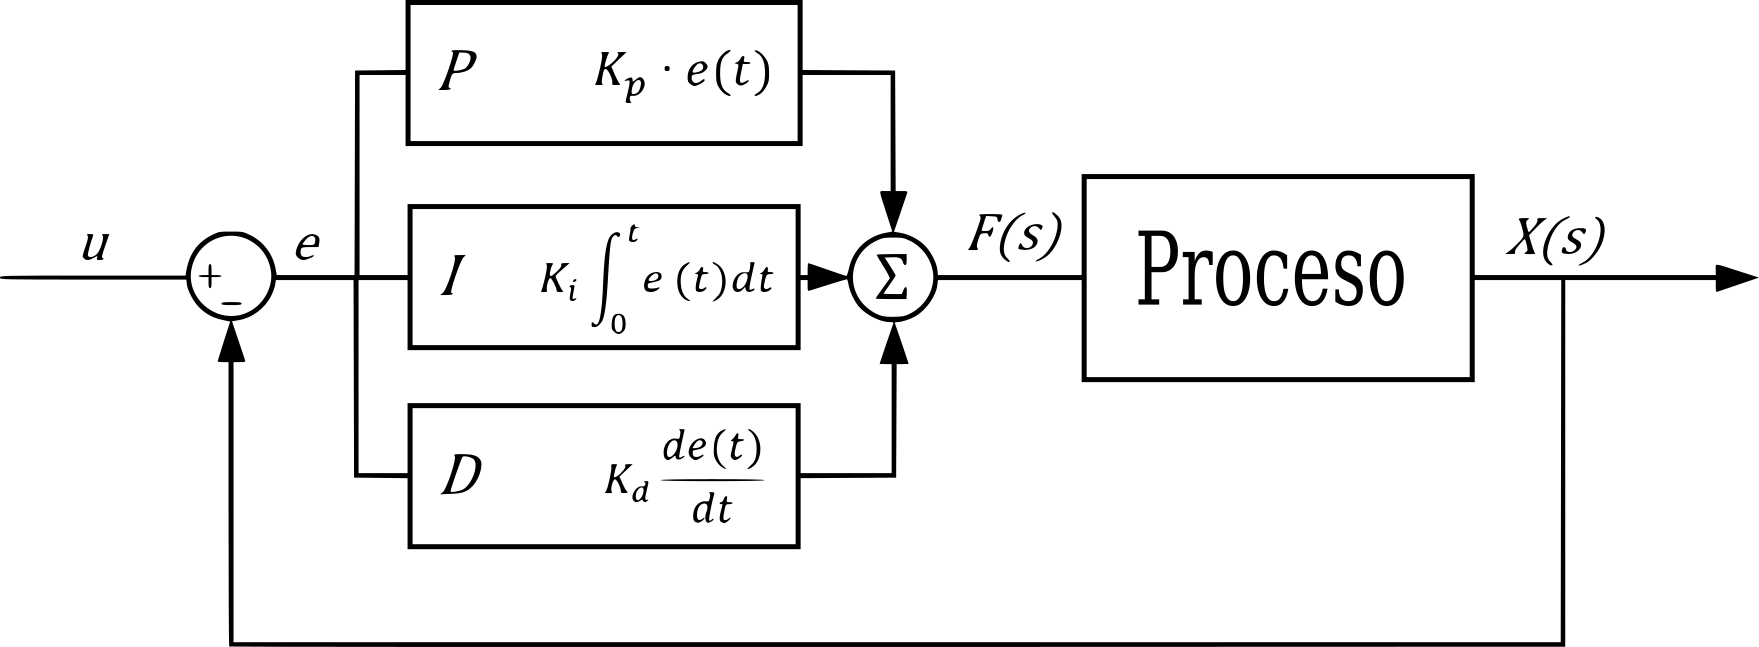
\includegraphics[width=0.5\textwidth]{./Figuras/PID}
	\caption{Diagrama de bloques para un controlador PID.}
	\label{fig:PID}
\end{figure}
\par En la expresión matemática para un controlador PID cada coeficiente ($K_{p}$, $K_{i}$, $K_{d}$) necesita ser sintonizado. Ahora, la expresión matemática para una controlador PID es la siguiente:
\[u(t)=K_{p}e(t)+K_{i}\int_{0}^{t}e(\tau)d\tau+K_{d}\frac{de(t)}{dt}\]
\par Para el problema que se aborda en este trabajo también se han encontrado en la bibliografía enfoques usando {\it Control Predictivo Basado en Modelo (MPC)} o {\it Control Óptimo}, principalmente. 
\subsection{Control con realimentación visual}
Este trabajo se centra en la navegación reactiva a través de ambientes desconocidos, por lo que una vez obtenidas las directivas por parte del sistema de visión, es necesario pasarlas al sistema de control; es una sinergia que en la bibliografía se aborda como {\it visual servoing}, sin embargo el mismo se encuentra documentado en su mayoría para su aplicación en manipuladores robóticos y en comparación son pocos los textos en los que se aborda el problema para la robótica móvil. Partiendo de la metodología empleada por estos últimos es que se desarrolla esta sección.
\par En términos generales, el control con realimentación visual implica tomar la información obtenida de los sistemas visuales presentes en la plataforma, y usarla para controlar el movimiento del robot. De manera particular, existen dos técnicas principales que se toman en cuenta al momento de realizar el control visual: IBVS\footnote{Control visual basado en imagen.} y PBVS\footnote{Control visual basado en posición.}. 
\subsubsection{IBVS}
Se trata de un enfoque de control aplicado a la robótica, está basado en tareas definidas visualmente en coordenadas cartesianas con las características del entorno. A partir de esto se pueden definir los errores de aproximación y orientación para el IBVS como
\begin{subequations}
	\begin{equation}\label{eq:eibvs}
		e_{IBVS}=\sqrt{\dot{x}^{2}+\dot{y}^2}
	\end{equation}
	\begin{equation}\label{eq:dibvs}
		\delta_{IBVS}=\arctan\left(\frac{\dot{y}}{\dot{x}}\right)
	\end{equation}
\end{subequations} 
teniendo a $\dot{x}$  y a $\dot{y}$ como las componente en $x$ e $y$ de la velocidad instantánea del RMR.
\begin{figure}[htbp!]
	\centering
	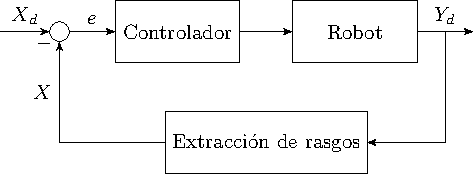
\includegraphics[width=0.5\textwidth]{./Figuras/IBVS/IBVS}
	\caption{Control visual basado en IBVS.}
	\label{fig:IBVS}
\end{figure}
\par A partir de estos dos parámetros es suficiente para estimar la ubicación del robot de manera planar. En el control basado en IBVS las características de la imagen son usadas directamente como realimentación en el sistema, con lo cual puede reducir el retraso en el cálculo, además de eliminar la necesidad de interpretación de la imagen y eliminar errores causados por la calibración de la imagen. Sin embargo representa por sí mismo un reto para el diseño del controlador, esto debido a que se cuenta con una proceso no lineal. Un diagrama de bloques que representa al IBVS se puede encontrar en la Figura \ref{fig:IBVS}.
\subsubsection{PBVS}
El diagrama de bloques para un sistema de control basado en PBVS se observa en la Figura \ref{fig:PBVS}. En el control basado en PBVS las características son extraídas de la imagen y son usadas en conjunto con el modelo geométrico del objetivo y en la posición estimada de la cámara. La realimentación es calculada al reducir el error en el espacio de configuraciones estimado.
En el control basado en PBVS los errores se calculan de manera planar como
\begin{subequations}
	\begin{equation}\label{eq:epbvs}
		e_{PBVS}=\sqrt{\dot{x}^{2}+\dot{y}^2}
	\end{equation}
	\begin{equation}\label{eq:dpbvs}
		\delta_{PBVS}=\theta_{d}-\theta
	\end{equation}
\end{subequations}
teniendo a $\dot{x}$ e $\dot{y}$ como las componentes $x$ e $y$ de la velocidad instantánea, respectivamente, $\theta_{d}$ como la orientación deseada y $\theta$ como la orientación actual.
\par Los componentes $e_{IBVS}$, $\delta_{IBVS}$, $e_{PBVS}$ y $\delta_{PBVS}$ deben pertenecer a la interacción del plano de la imagen con el espacio de trabajo. A esa interacción se le conoce como matriz Jacobiana, y su resultado son los componentes $\dot{x}$ e $\dot{y}$.
\begin{figure}[htbp!]
	\centering
	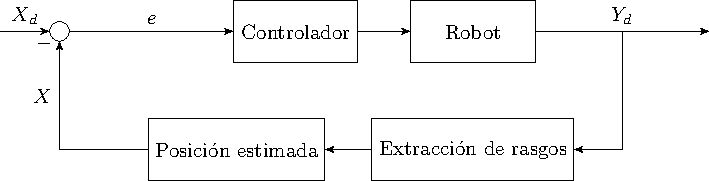
\includegraphics[width=0.5\textwidth]{./Figuras/PBVS/PBVS}
	\caption{Control visual basado en PBVS.}
	\label{fig:PBVS}
\end{figure}